\documentclass[12pt, centerh1]{article}
\textwidth=165mm \headheight=0mm \headsep=10mm \topmargin=-10mm
\textheight=230mm %\footskip=1.5cm
\oddsidemargin=0mm
%\documentclass[12pt,letterpaper]{article}
%\usepackage[margin=1in]{geometry}
\RequirePackage[colorlinks,citecolor=blue,urlcolor=blue]{hyperref}
\usepackage{amsmath, amssymb,natbib}
%\usepackage[mathscr]{euscript}
%\usepackage{mathrsfs}
\usepackage{graphicx,bm}
\usepackage{color}
\usepackage{subcaption}
\usepackage{subcaption}
\usepackage[table]{xcolor}
\usepackage{longtable}
\usepackage{amsthm}
\usepackage[mathscr]{euscript}
\usepackage{relsize}
\usepackage{amsmath,tabularx}
\newcolumntype{P}[1]{>{\centering\arraybackslash}p{#1}}
\usepackage{rotating}
\usepackage{eurosym}
\usepackage{colonequals}
\usepackage{bbm}
\usepackage{lscape}
\usepackage{natbib}

%%% make comments using the following setup %%
% type \your name {comment}, 
% e.g. \sophie{i love lyme disease}
\newcommand{\bruce}[1]{{\textcolor{blue}{$\langle$BC: #1$\rangle$}}}
\newcommand{\sophie}[1]{{\textcolor{purple}{$\langle$SS: #1$\rangle$}}}
\newcommand{\lauren}[1]{{\textcolor{cyan}{$\langle$LF: #1$\rangle$}}}
\newcommand{\geneva}[1]{{\textcolor{green}{$\langle$GL: #1$\rangle$}}}
\newcommand{\thanesh}[1]{{\textcolor{yellow}{$\langle$TR: #1$\rangle$}}}

\title{We care about acaricide $<3$}

%%% put in alphabetical order
\author{\qquad name$^{1,3}$ \qquad\  name$^{1}$ \qquad\  name$^{1,3}$ \\  name$^{2}$ \quad\ Sophie Stelmach$^{1}$}

\date{{\small $^1$ Department of Mathematics \& Statistics, McMaster University, Ontario, Canada.\\[-6pt]
$^2$ add your institution\\[-6pt]
$^3$ \\[-6pt]
}
}
\linespread{1.5}
\pdfminorversion=4

\begin{document}

% makes title
\maketitle



\section{Introduction}
Lyme disease is a highly emerging vector-borne disease in North America, which is caused by the bacterium \textit{Borrelia} and transmitted via infected bites of black-legged ticks (\textit{Ixodes}) \citep{govcan}. The risk of disease is further propagated by the changes in migratory patterns northward of these ticks by climate change.

\textbf{\textit{Borrelia}}, particularly B. burgdorferi sensu lato

\textbf{Black-legged Tick}
I. scapularis is primary cause of LD in Eastern North America. I. scapularis is also a vector for many types of pathogens such as Borrelia mayonni, Powassan virus and Anaplasma phaocytophilum \citep{paulson2023multiomics}. This shows that besides Lyme disease, the black-legged tick can also increase the risk for poly microbial infections. 


\textbf{Lyme disease}
Lyme disease clinical manifestation can be divided into three stages; early localization, early dissemination and late persistence. 

\textbf{Lyme disease in Canada}
A study in eastern and southern Ontario, Canada found \textit{Borrelia} sp in approximately 70 percent of ticks with a relative abundance of 0.01 percent \citep{clow2018microbiota}. Concentration of adult \textit{I. scapularis} carrying endosymbiotic and pathogenic microorganisms in southeastern Ontario \citep{paulson2023multiomics}. 

In this study, a mathematical model was developed to evaluate the efficacy of acacides as a Lyme disease intervention during the tick larval growth stage in Ontario, Canada.




\begin{figure}[h]
    \centering
    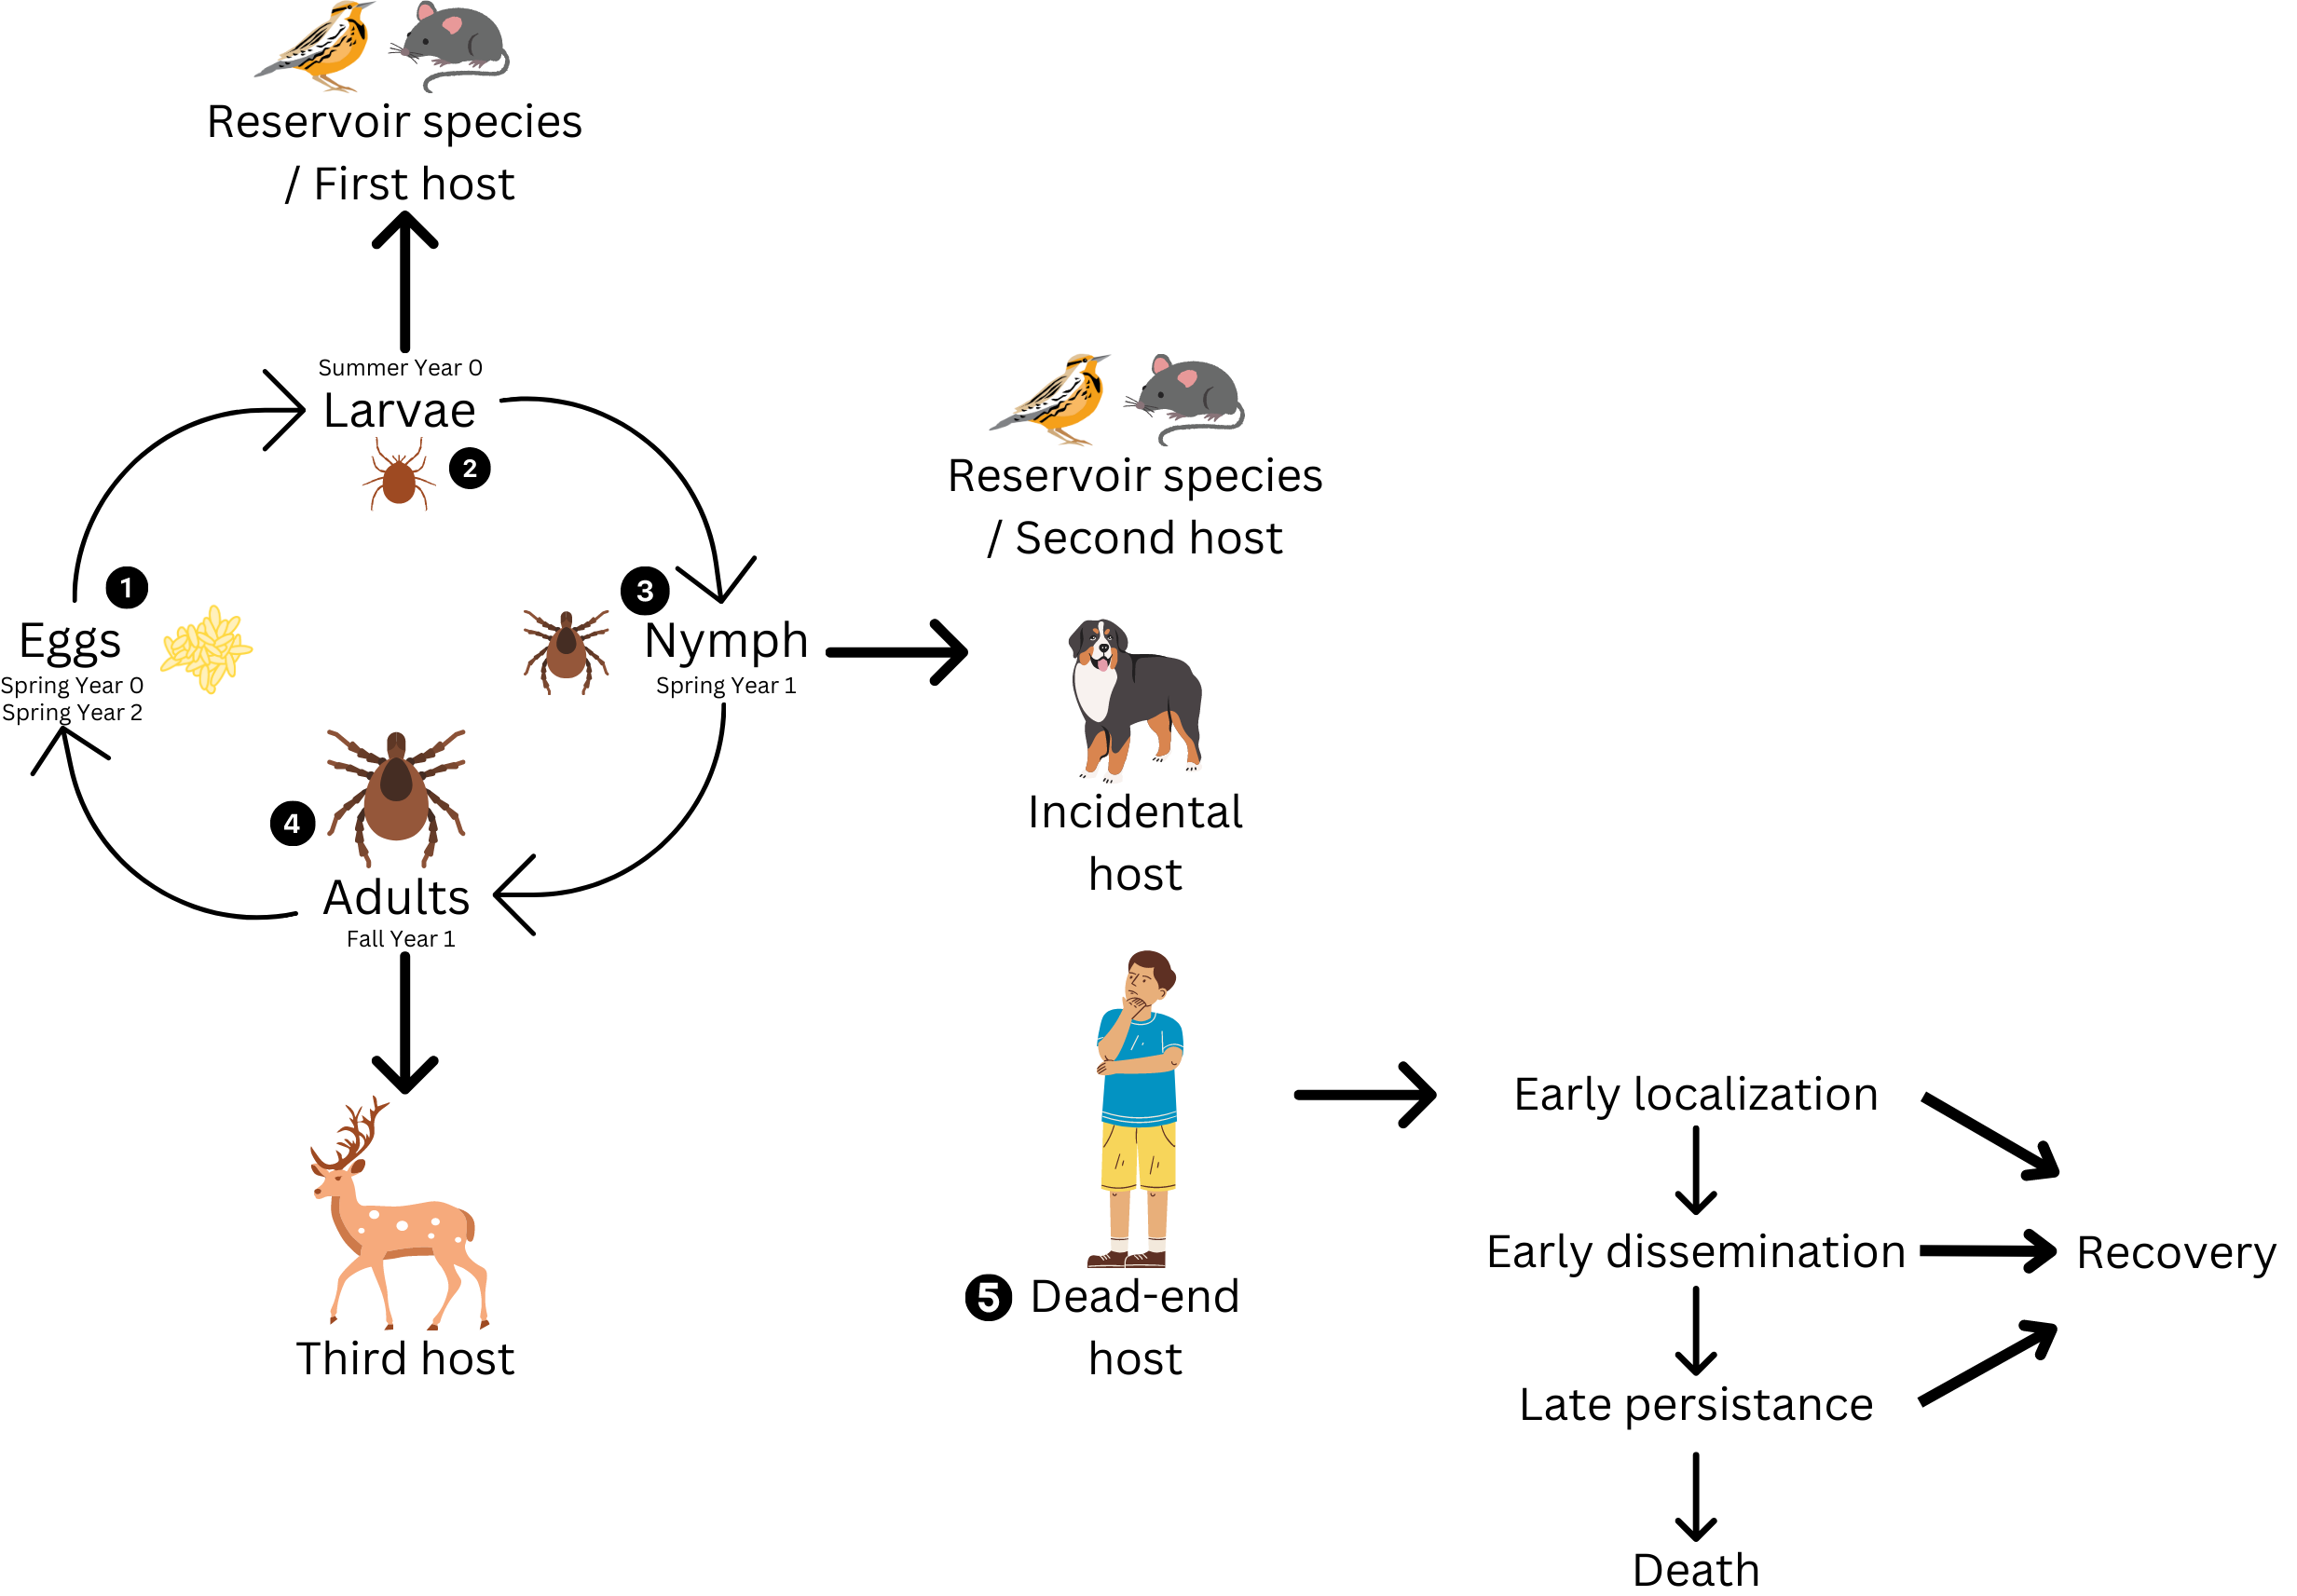
\includegraphics[scale = 0.15]{figures/Tick life cycle and progression of lyme disease.png}
    \caption{Diagram of tick life cycle and host bias.}
    \label{fig:lifecycle}
\end{figure}

\section{Methods}

\subsection{Proposed Model}
The model proposed by \citet{lou2014impact} describes the tick life cycle and disease transmission between the tick and its hosts. The model features fifteen compartments, thirteen of which represent the various stages of the tick life cycle, including healthy ticks and infected ticks. We will base our analysis on this model, adding an intervention to prevent Lyme disease spread, and simplify certain aspects of the model. 

Ticks feed on their hosts in the larva, nymph, and adult stages of the life cycle, but only pose a risk to humans in the late larval and early-to-mid nymph stage. During the larval stage, ticks will feel on small rodents, at which point they risk acquiring Lyme disease-causing bacteria \sophie{cite}. Nymphs and adults feed on their hosts at different rates, which is why the model features different feeding rates for each of these stages.
At each stage of the tick life cycle, we feature a mortality rate based on the values listed in \citet{lou2014impact}, which were found in previous publications. 

To avoid including unnecessary model complexity, we removed the time-dependent nature of the model 

\sophie{Lauren/whoever insert compartmental diagram here}

\subsection{Model Assumptions}
- assumptions
- dynamics?

\subsection{}


\section{Results}



\section{Discussion}

\subsection{Model Implications}

\subsection{Effect on Policy Decisions}

\subsection{Future Studies}


\section{Conclusion}

\newpage
\bibliographystyle{chicago} %idk what style we want to do
\bibliography{bib}
\end{document}